\setchapterstyle{kao}
\setchapterpreamble[u]{\margintoc}

\chapter{Beyond the Standard Model Neutrinos}
\labch{bsm_neutrinos}


\section{Neutrino Oscillations}

\subsection{Vacuum Oscillations}

\subsection{Oscillations in Matter}

% \subsection{Three-Flavor Oscillations}

\subsection{Atmospheric Neutrino Oscillations}

\subsubsection{Neutrino Production in the Atmosphere}

The flux of neutrinos used for this work exclusively comes from the Earth's atmosphere.
The nominal flux model is calculated by \sidecite{PhysRevD.92.023004_Honda_Flux} in the energy range of 100\,MeV to 10\,TeV.
When highly relativistic cosmic rays (protons and heavier nuclei \sidecite{PhysRevD.98.030001}) interact in  the upper atmosphere they produce a shower of particles. 
Neutrinos emerge from the decays of charged pions and kaons ($\pi$ and $K$ mesons) present in these showers.
For energies below 100\,GeV, the leading contribution comes from the pion decay chain
\begin{equation}
    \begin{split}   
        \pi^\pm &\rightarrow \mu^\pm + \nu_\mu(\bar{\nu}_\mu), \\
        \mu^\pm &\rightarrow e^\pm + \bar{\nu}_\mu(\nu_\mu) + \nu_e(\bar{\nu}_e).
    \end{split}
    \labeq{pion_decay}
\end{equation}
The muons that also originate from this process are considered the main background source for IceCube.
The left part of Figure \reffig{honda_flux} shows the atmospheric neutrino flux for the very broad energy spectrum in which they are produced.
The flux expectations are calculated for the South Pole \sidecite{PhysRevD.92.023004_Honda_Flux}, where the IceCube detector is located.
From Equation \refeq{pion_decay} the ratio between muon and electron neutrinos can be inferred to be $N_{\nu_\mu}:N_{\nu_e} \approx 2:1$.
This is only the case at muon energies below 1\,GeV, where all muons decay in flight.
For higher energies, muons can reach earth before decaying increasing the ratio to approximately 10:1 at around 100\,GeV as shown in the right part of Figure \reffig{honda_flux}.
Additionally, kaon decays start to contribute which also increases the number of muons and muon neutrinos.

\begin{figure}[h]
    \centering
    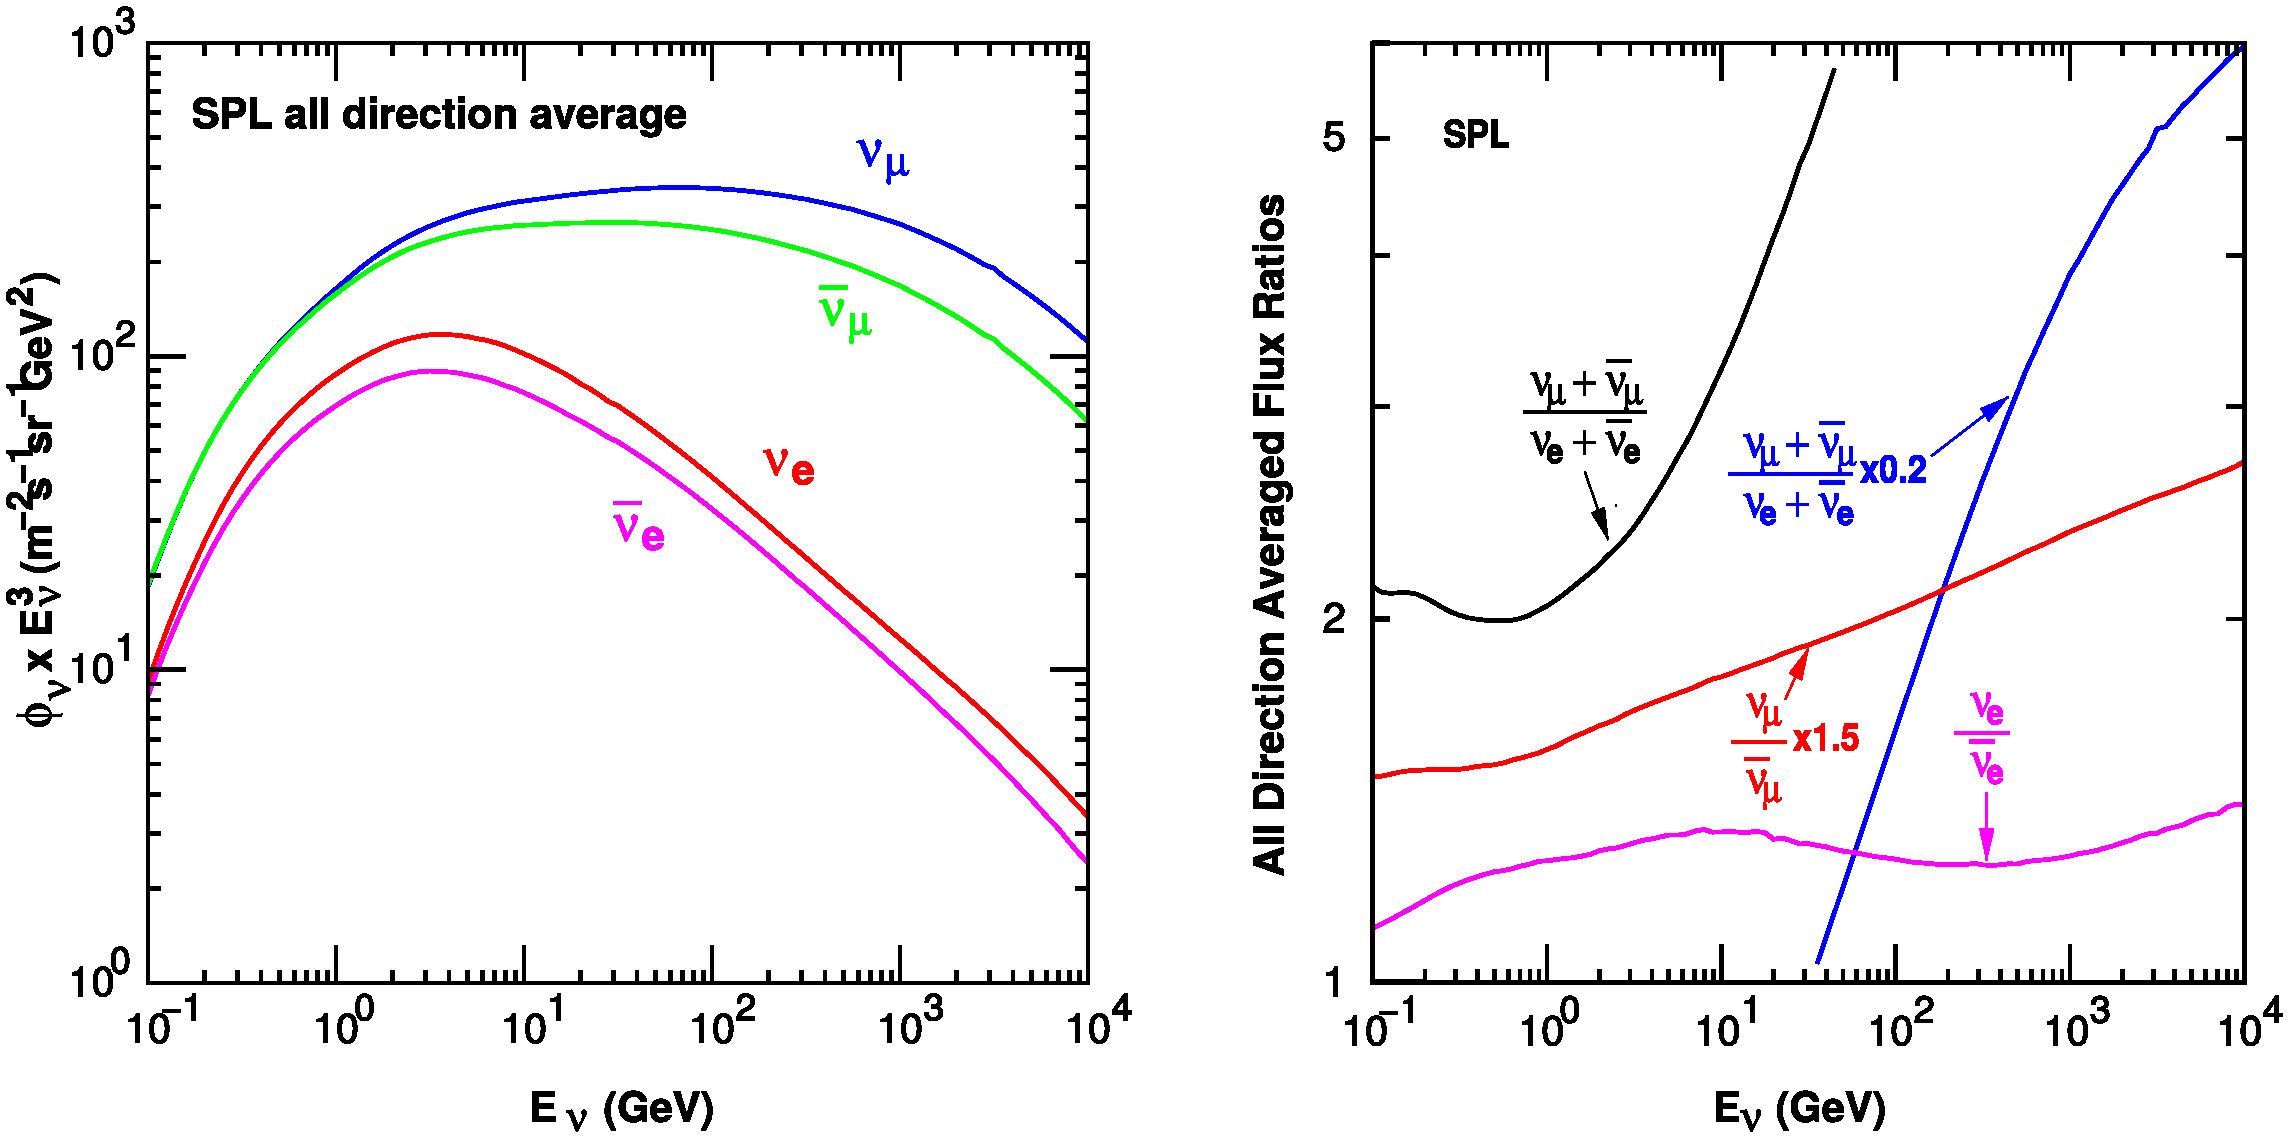
\includegraphics[width=1.0\textwidth]{figures/neutrinos_properties/Honda_alldir-spl_copy.pdf}
    \caption[Atmospheric neutrino fluxes, taken from \cite{PhysRevD.92.023004_Honda_Flux}]{Atmospheric neutrino fluxes of the different flavors as a function of energy (left) and ratios between muon- and electron-neutrinos as well as ratios between neutrinos and antineutrinos for both flavors (right). Calculations are done for the geographic South Pole. Taken from \cite{PhysRevD.92.023004_Honda_Flux}.}
    \label{fig:honda_flux}
\end{figure}

In cosmic ray interactions, charged mesons or tau particles can also be produced, which leads to the formation of tau neutrinos.
However, at the energy range considered for this work, the resulting tau neutrino flux is negligible as compared to the muon neutrino flux \sidecite{2015EPJWC..9908001F_lepton_fluxes} and is not taken into account.
% is less than 0.1\,\%  of the muon neutrino flux and can, therefore, be neglected.
It should be stated here that there is a rather large uncertainty on the normalization of the atmospheric neutrino flux on the order of 20-30\,\% \sidecite{PhysRevD.75.043006_neutino_flux_honda} in the energy region of interest.
This is mainly due to uncertainties in the primary cosmic ray spectrum and modeling of the hadronic interactions.


\subsubsection{Oscillations of Atmospheric Neutrinos}

There are two ways to describe neutrino wave functions based on their Hamiltonian eigenvalues \sidecite{BILENKY1978225}, as mass eigenstates or as flavor eigenstates.
When applying a plane wave approach to explain the propagation of neutrinos in vacuum, their mass eigenstates evolve as
\begin{equation}
    \ket{\nu_k(t)} = e^{-iE_kt/\hbar}\ket{\nu_k},
    \labeq{flavor_time_evol}
\end{equation}
where $E_k=\sqrt{\vec{p}^2c^2+m_k^2c^4}$ is the energy of the mass eigenstate $\ket{\nu_k}$, with momentum $\vec{p}$ and mass $m_k$.
Alternatively, they can be described in terms of their flavor eigenstates, which relate the neutrinos to the charged leptons they interact with in weak CC interactions.
The flavor eigenstates are $\nu_e, \nu_\mu$, and $\nu_\tau$, whereas the mass eigenstates are called $\nu_1, \nu_2$, and $\nu_3$ in the standard three-neutrino model.
To understand the propagation of distinct neutrino flavors in time (in vacuum) we need to relate the flavor eigenstates to the mass eigenstates.
For massive neutrinos, each flavor eigenstate is a superposition of mass eigenstates \sidecite{PhysRevD.98.030001}
\begin{equation}
    \ket{\nu_\alpha} = \sum_kU^*_{\alpha k}\ket{\nu_k},
    \labeq{neutrino_mixing}
\end{equation}
where $\ket{\nu_\alpha}$ are the weak flavor states with $\alpha=e,\mu,\tau$ and $\ket{\nu_k}$ the mass states with $k=1,2,3$.
$U_{\alpha k}$ is the Pontecorvo-Maki-Nakagawa-Sakata (PMNS) matrix defining the mixing between mass and flavor eigenstates.
The mixing matrix can be parameterized as \sidecite{PhysRevD.98.030001}
\begin{equation}
    U=\left( 
    \begin{matrix}
        1 & 0 & 0 \\
        0 & c_{23}  & s_{23} \\
        0 & -s_{23} & c_{23} 
    \end{matrix}
    \right) 
    \left( 
    \begin{matrix}
        c_{13} & 0 & s_{13}e^{-i\delta_{CP}} \\
        0 & 1 & 0\\
        -s_{13} e^{i\delta_{CP}} & 0 & c_{13}
    \end{matrix}
    \right) 
    \left( 
    \begin{matrix}
        c_{12} & s_{12} & 0 \\
        -s_{12} & c_{12} & 0\\
        0 & 0 & 1
    \end{matrix} 
    \right)  
    \operatorname{diag}(e^{i\rho_{1}},e^{i\rho_{2}},1),
    \labeq{PMNS_matrix}
\end{equation}
where $c_{ij}=\cos\theta_{ij}$ and $s_{ij}=\sin\theta_{ij}$ are cosine and sine of the mixing angle $\theta_{ij}$, that defines the strength of the mixing between the mass eigenstates i and j and $\delta_{CP}$ is the neutrino CP-violating phase.
Nonzero, non-equal neutrino masses and the neutrino mixing relation in Equation \refeq{neutrino_mixing} lead to the observed phenomenon of neutrino oscillations.
Oscillation means that a neutrino changes from its initial flavor to another flavor and back after traveling a certain distance.
A produced flavor eigenstate $\ket{\nu_\alpha}$ propagates through space as a superposition of mass eigenstates.
To find the probability that the initial flavor state $\ket{\nu_\alpha}$ ends up as the final flavor state $\ket{\nu_\beta}$ after the time $t$ we calculate
\begin{equation}
    P_{\nu_\alpha \rightarrow \nu_\beta}(t)
    =
    |\braket{\nu_\beta|\nu_\alpha(t)}|^2,
    \labeq{fermis_golden_rule}
\end{equation}
where $P$ is the probability calculated by applying Fermi's Golden Rule \sidecite{1927RSPSA.114..243D}.
Fermi's Golden Rule explains the transition rate from one energy eigenstate to another depending on the strength of the coupling between the two.
The strength of the coupling is described by the square of the matrix element.
Using the unitarity of the mixing matrix $U^{-1}=U^\dagger$ to reverse the relation \refeq{neutrino_mixing} and then time evolve the mass eigenstates with Equation \refeq{flavor_time_evol} we get the time evolution of the flavor state $\ket{\nu_\alpha(t)}$.
Inserting this result into Equation \refeq{fermis_golden_rule} yields
\begin{equation}
    P_{\nu_\alpha \rightarrow \nu_\beta}(t)
    =
    \sum_{j,k}U^*_{\beta j}U_{\alpha j}U_{\beta k}U^*_{\alpha k}e^{-i(E_k-E_j)t/\hbar},
    \labeq{probability_raw}
\end{equation}
where the indices $j$ and $k$ run over the mass eigenstates. For small neutrino masses compared to their kinetic energy, we can approximate the energy as
\begin{equation}
    E_k \approx E+\frac{c^4m^2_k}{2E} \hspace{0.25cm} \longrightarrow \hspace{0.25cm} E_k-E_j \approx \frac{c^4\Delta m^2_{kj}}{2E},
\end{equation}
where $\Delta m^2_{kj}=m^2_k-m^2_j$ is the mass-squared splitting between states $k$ and $j$.
If we now replace the time in Equation \refeq{probability_raw} by the distance traveled by the relativistic neutrinos $t\approx L/c$ we get
\begin{equation}
    \begin{split}
        P_{\nu_\alpha \rightarrow \nu_\beta}(t)
        = 
        \delta_{\alpha \beta}
        -
        4\sum_{j>k}&\textbf{Re}(U^*_{\beta j}U_{\alpha j}U_{\beta k}U^*_{\alpha k})\textrm{sin}^2\Big( \frac{c^3\Delta m^2_{kj}}{4E\hbar}L \Big) \\
        +
        2\sum_{j>k}&\textbf{Im}(U^*_{\beta j}U_{\alpha j}U_{\beta k}U^*_{\alpha k})\textrm{sin}^2\Big( \frac{c^3\Delta m^2_{kj}}{4E\hbar}L \Big),
    \end{split}
    \labeq{probability_detailed}
\end{equation}
which is referred to as the survival probability if $\alpha=\beta$ and the transition probability if $\alpha\neq\beta$.
The probability in Equation \refeq{probability_detailed} is only nonzero if there are neutrino mass eigenstates with masses greater than zero.
Additionally, there must be a mass-squared difference $\Delta m^2$ and nonzero mixing between the states.
Since we assumed propagation in vacuum in Equation \refeq{flavor_time_evol}, the transition and survival probabilities correspond to vacuum mixing.


\subsubsection{Matter Effects}

% \subsection{Solar neutrinos}
% \subsection{Reactor neutrinos}
% \subsection{Accelerator neutrinos}
% \subsection{Anomalies in Neutrino Oscillation Measurements}


\section{Heavy Neutral Leptons}

\subsection{Motivation for Heavy Sterile Neutrinos}

\subsection{Extending the Standard Model}

% taken from technote
% \begin{figure}[h]
%     \subfloat[\labfig{hnl_decay_modes_log_branching_ratio}]{
%         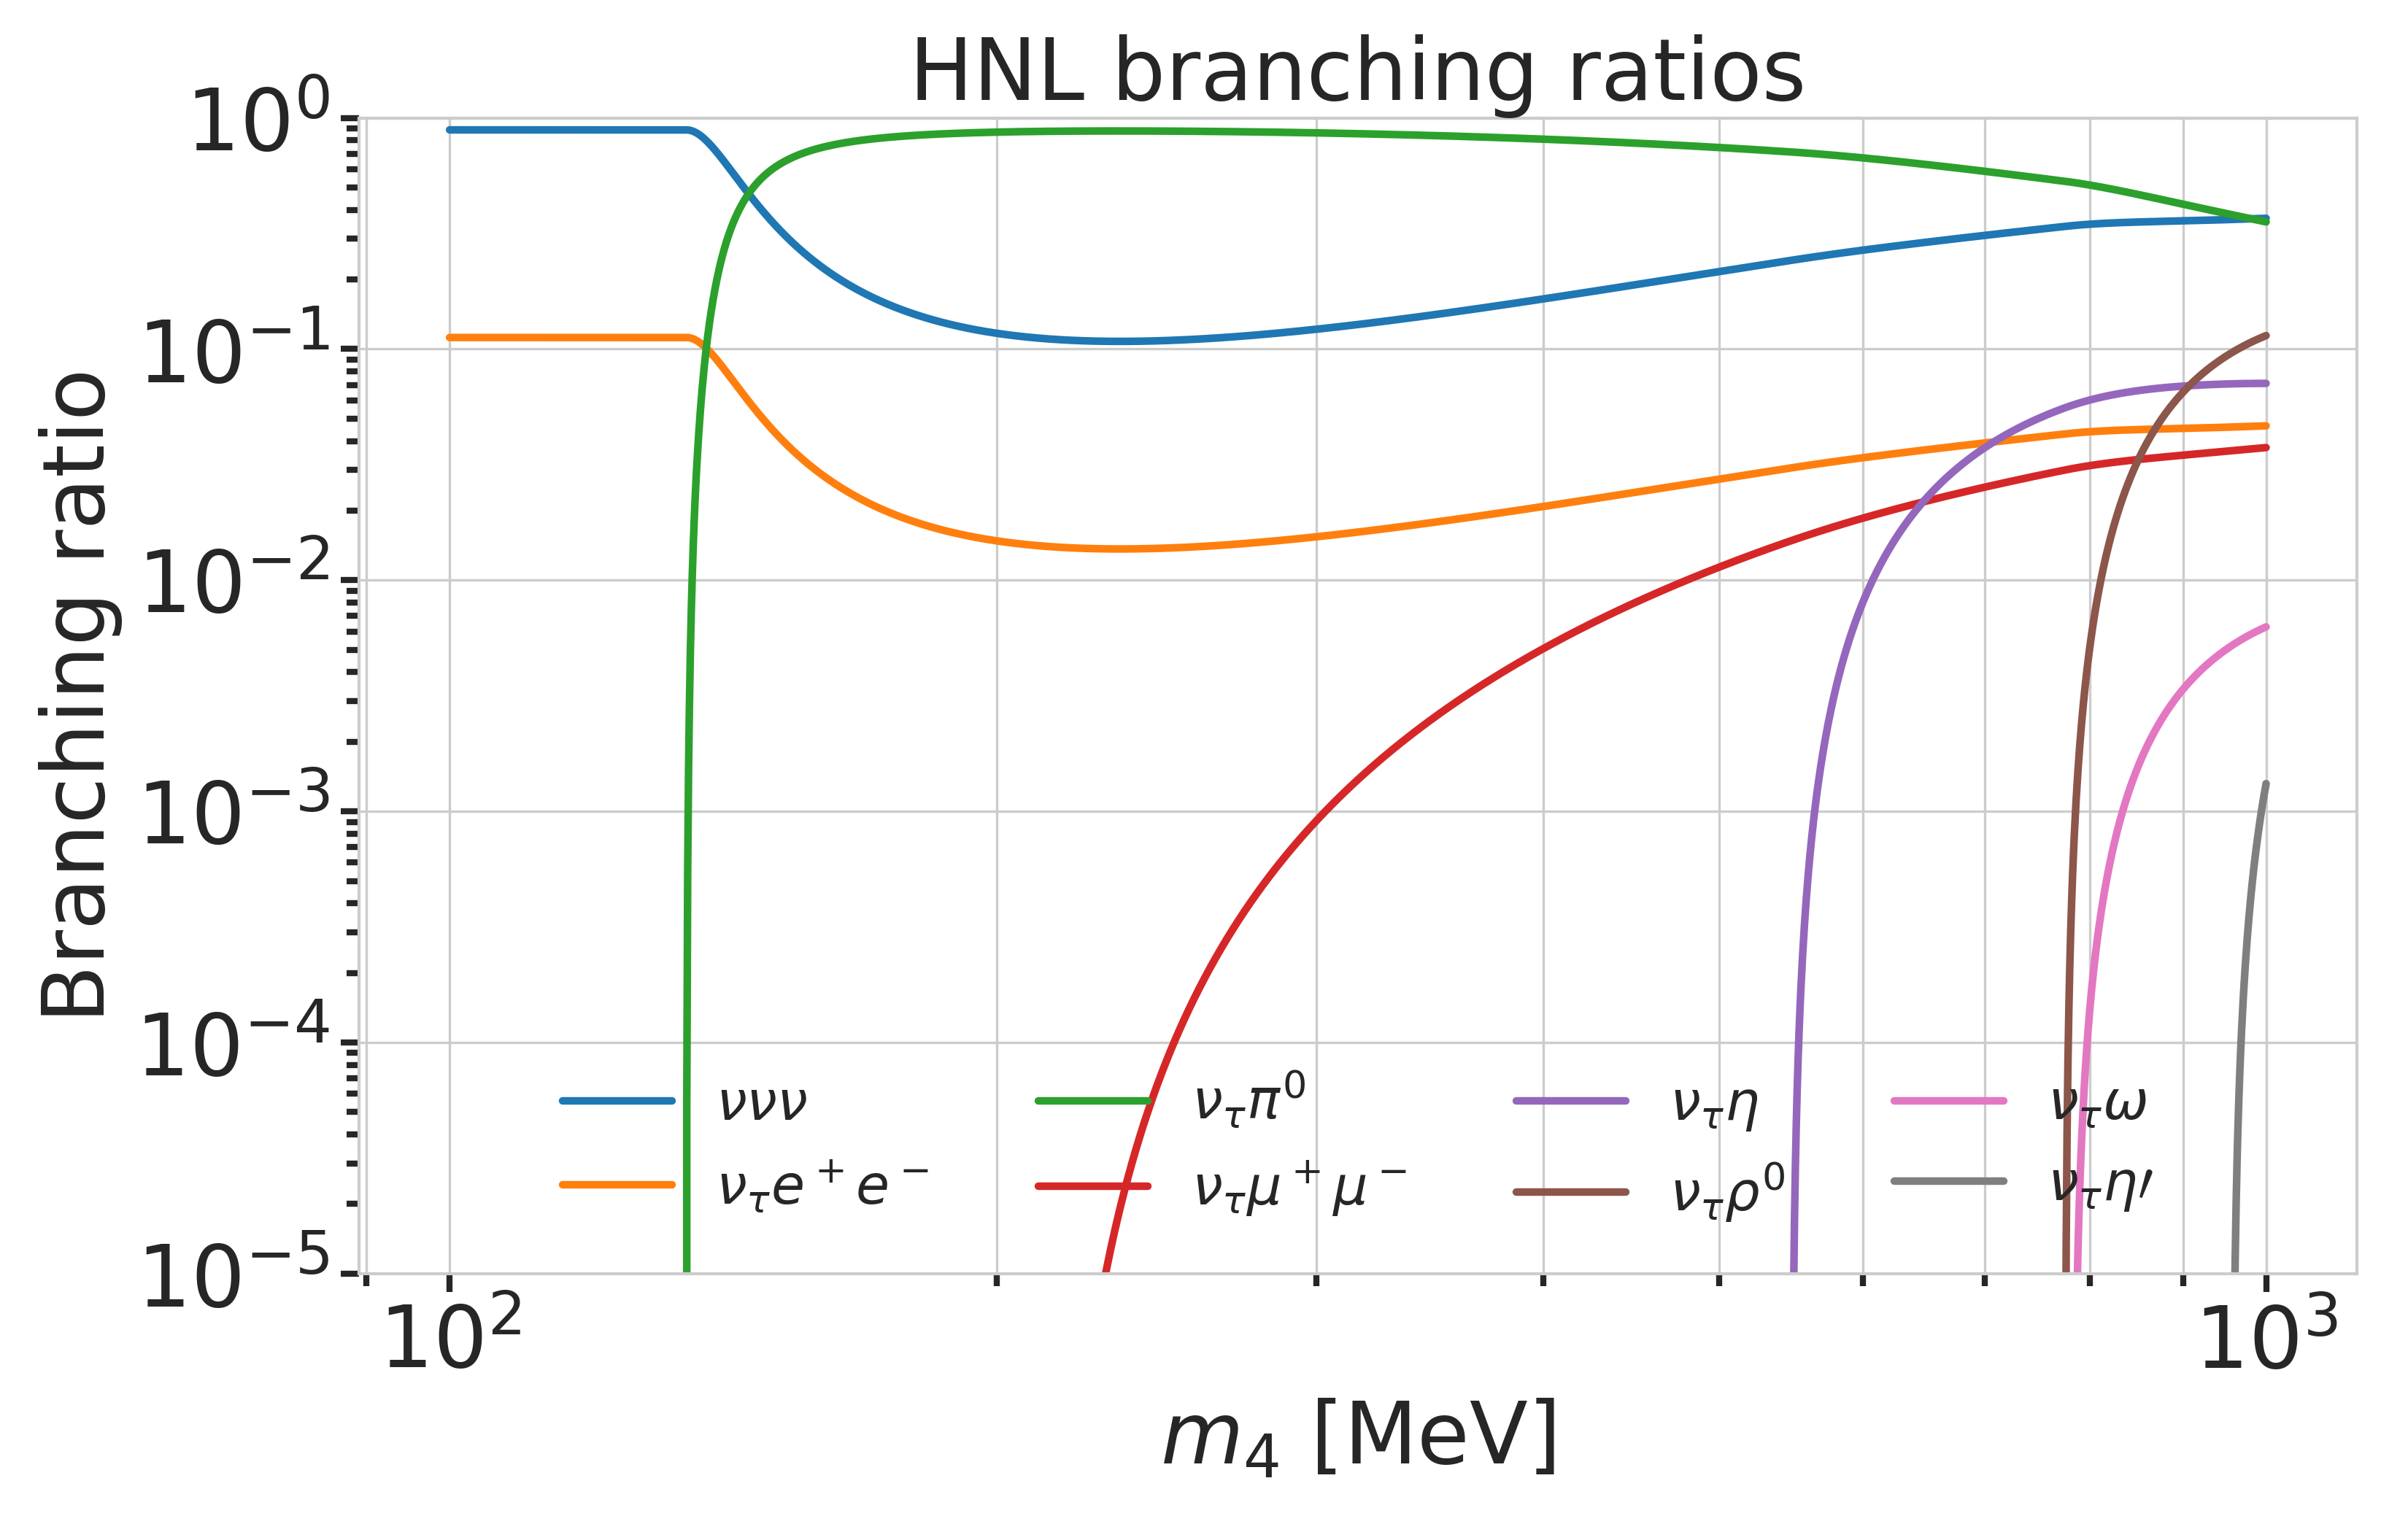
\includegraphics[width=.45\linewidth]{hnl_simulation/decay_theory/branching_ratios_log_up_to_1.0_GeV.png}
%     }
%     \subfloat[\labfig{hnl_decay_modes_log_decay_width}]{
%         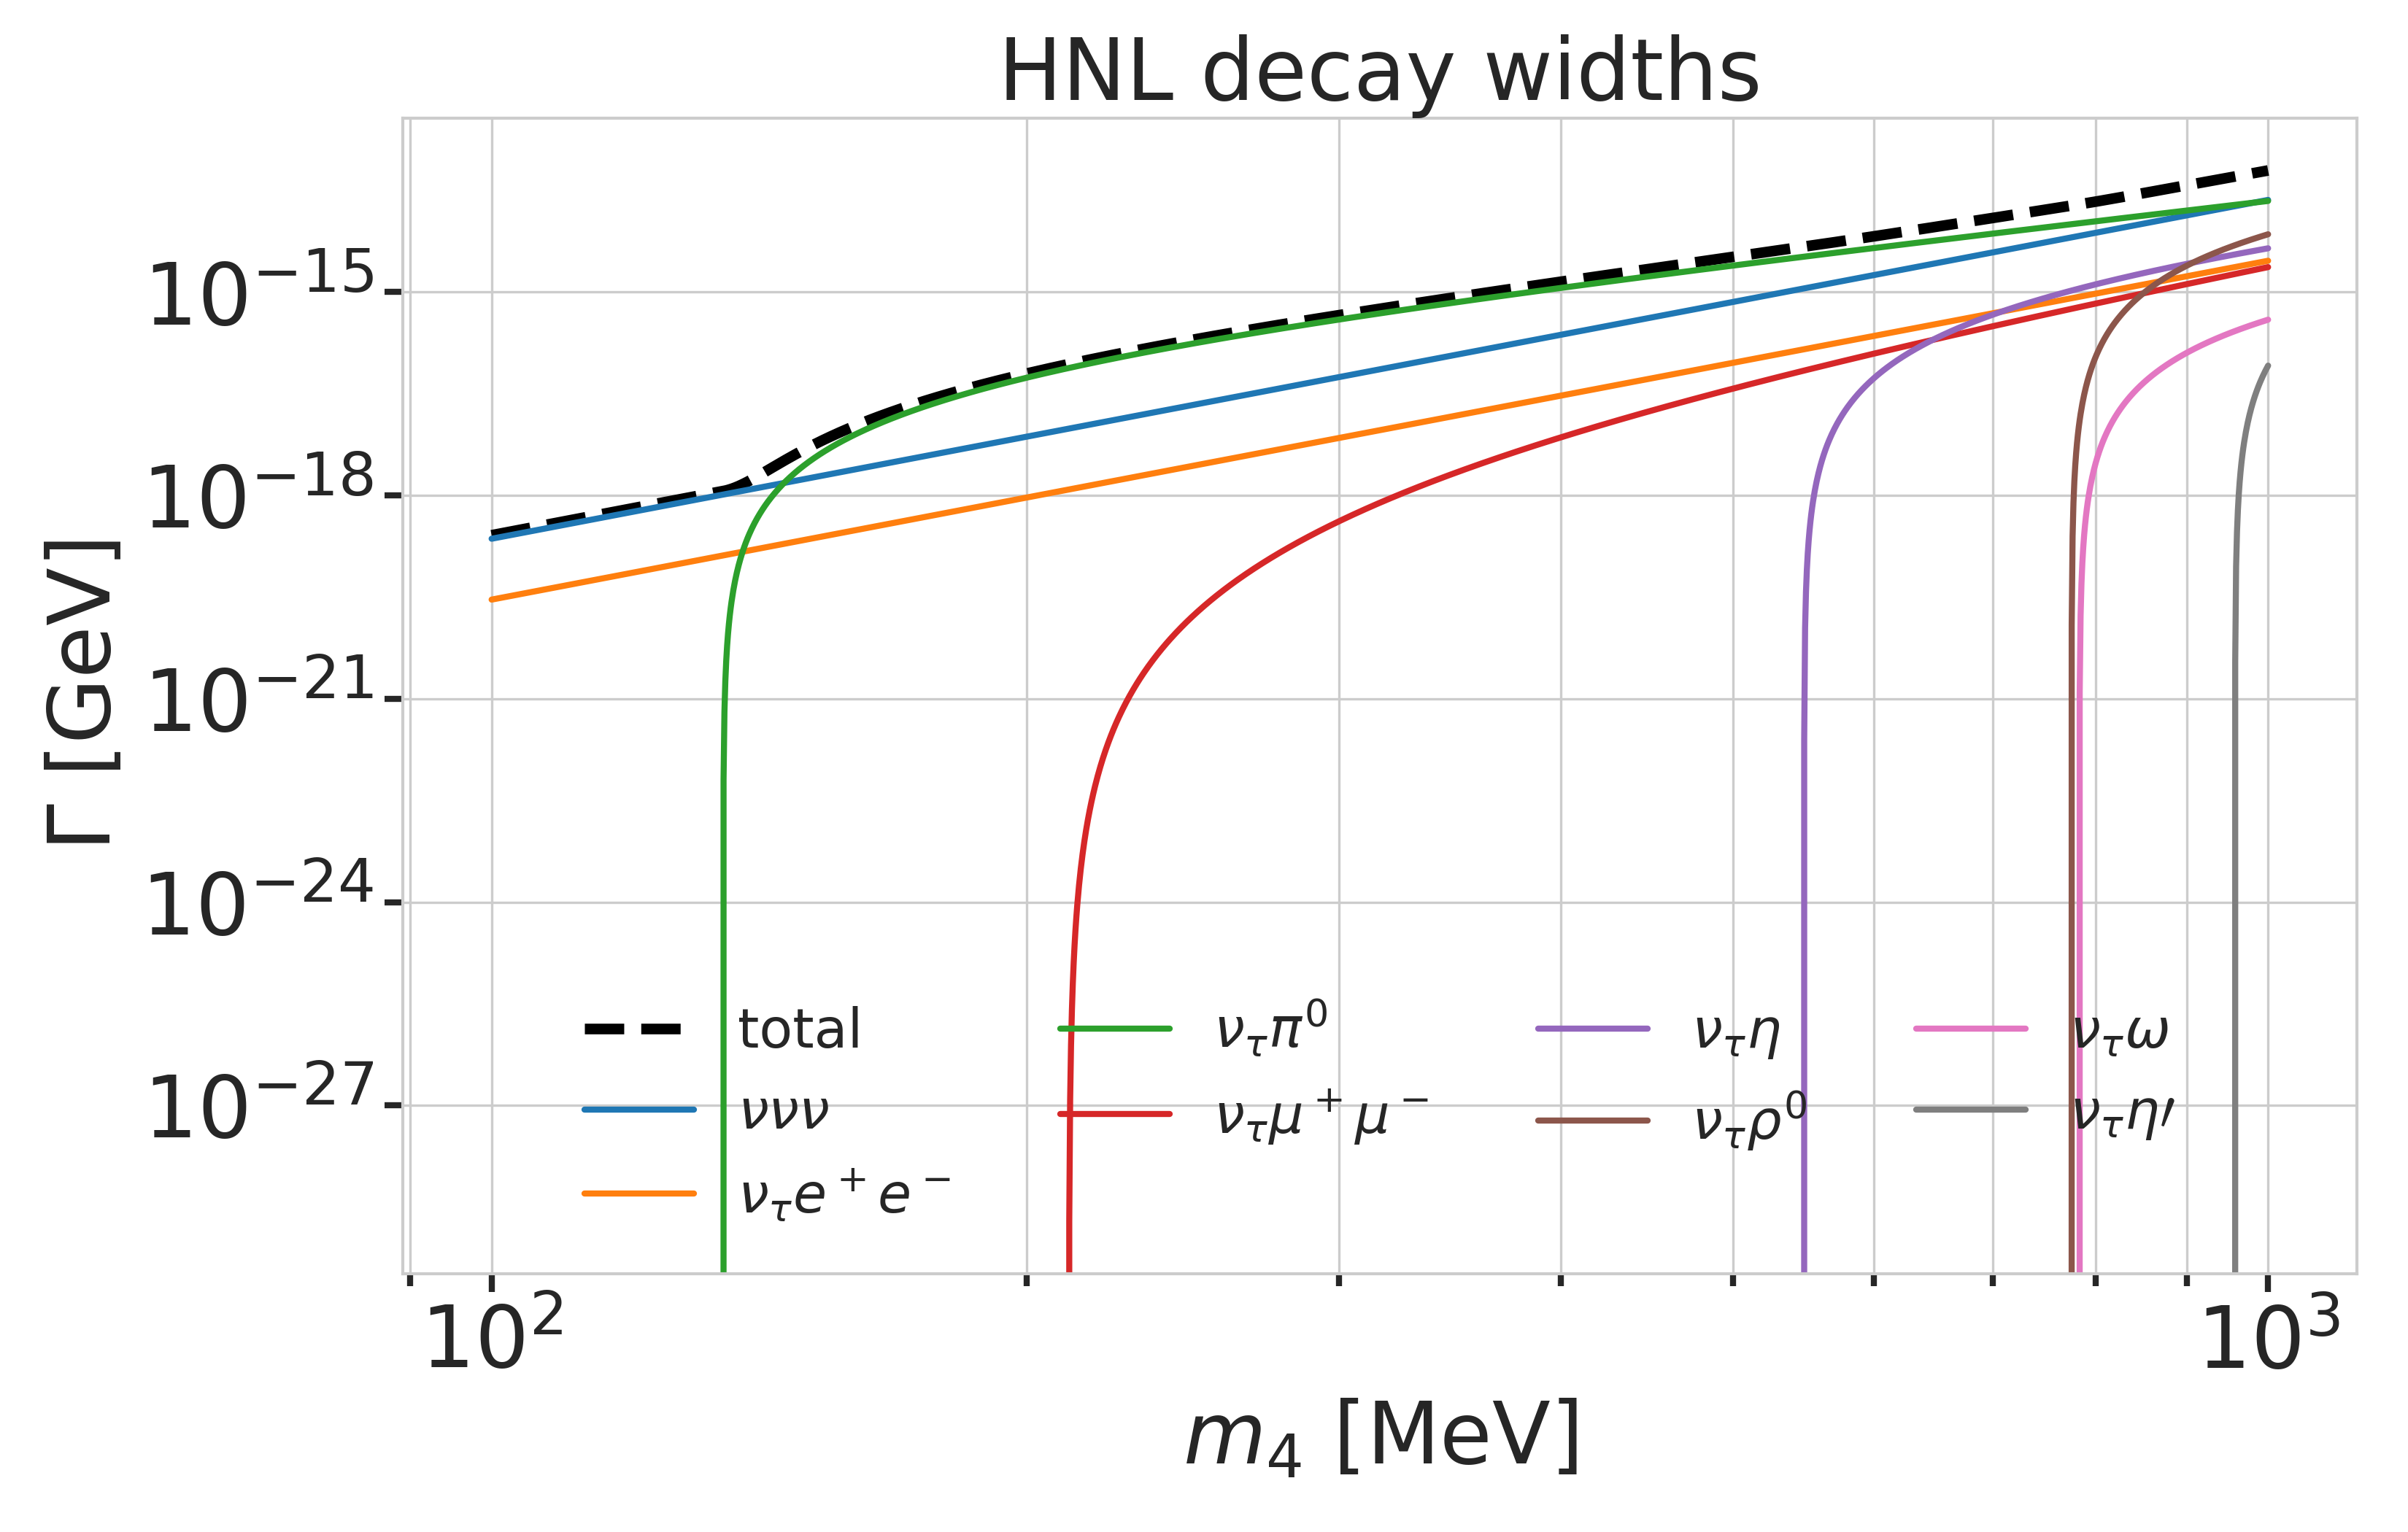
\includegraphics[width=.45\linewidth]{hnl_simulation/decay_theory/hnl_decay_widths_up_to_1.0_GeV_log.png}
%     }
%     \\[-2.5ex]
%     \centering
%     \subfloat[\labfig{hnl_decay_modes_log_proper_lifetime}]{
%         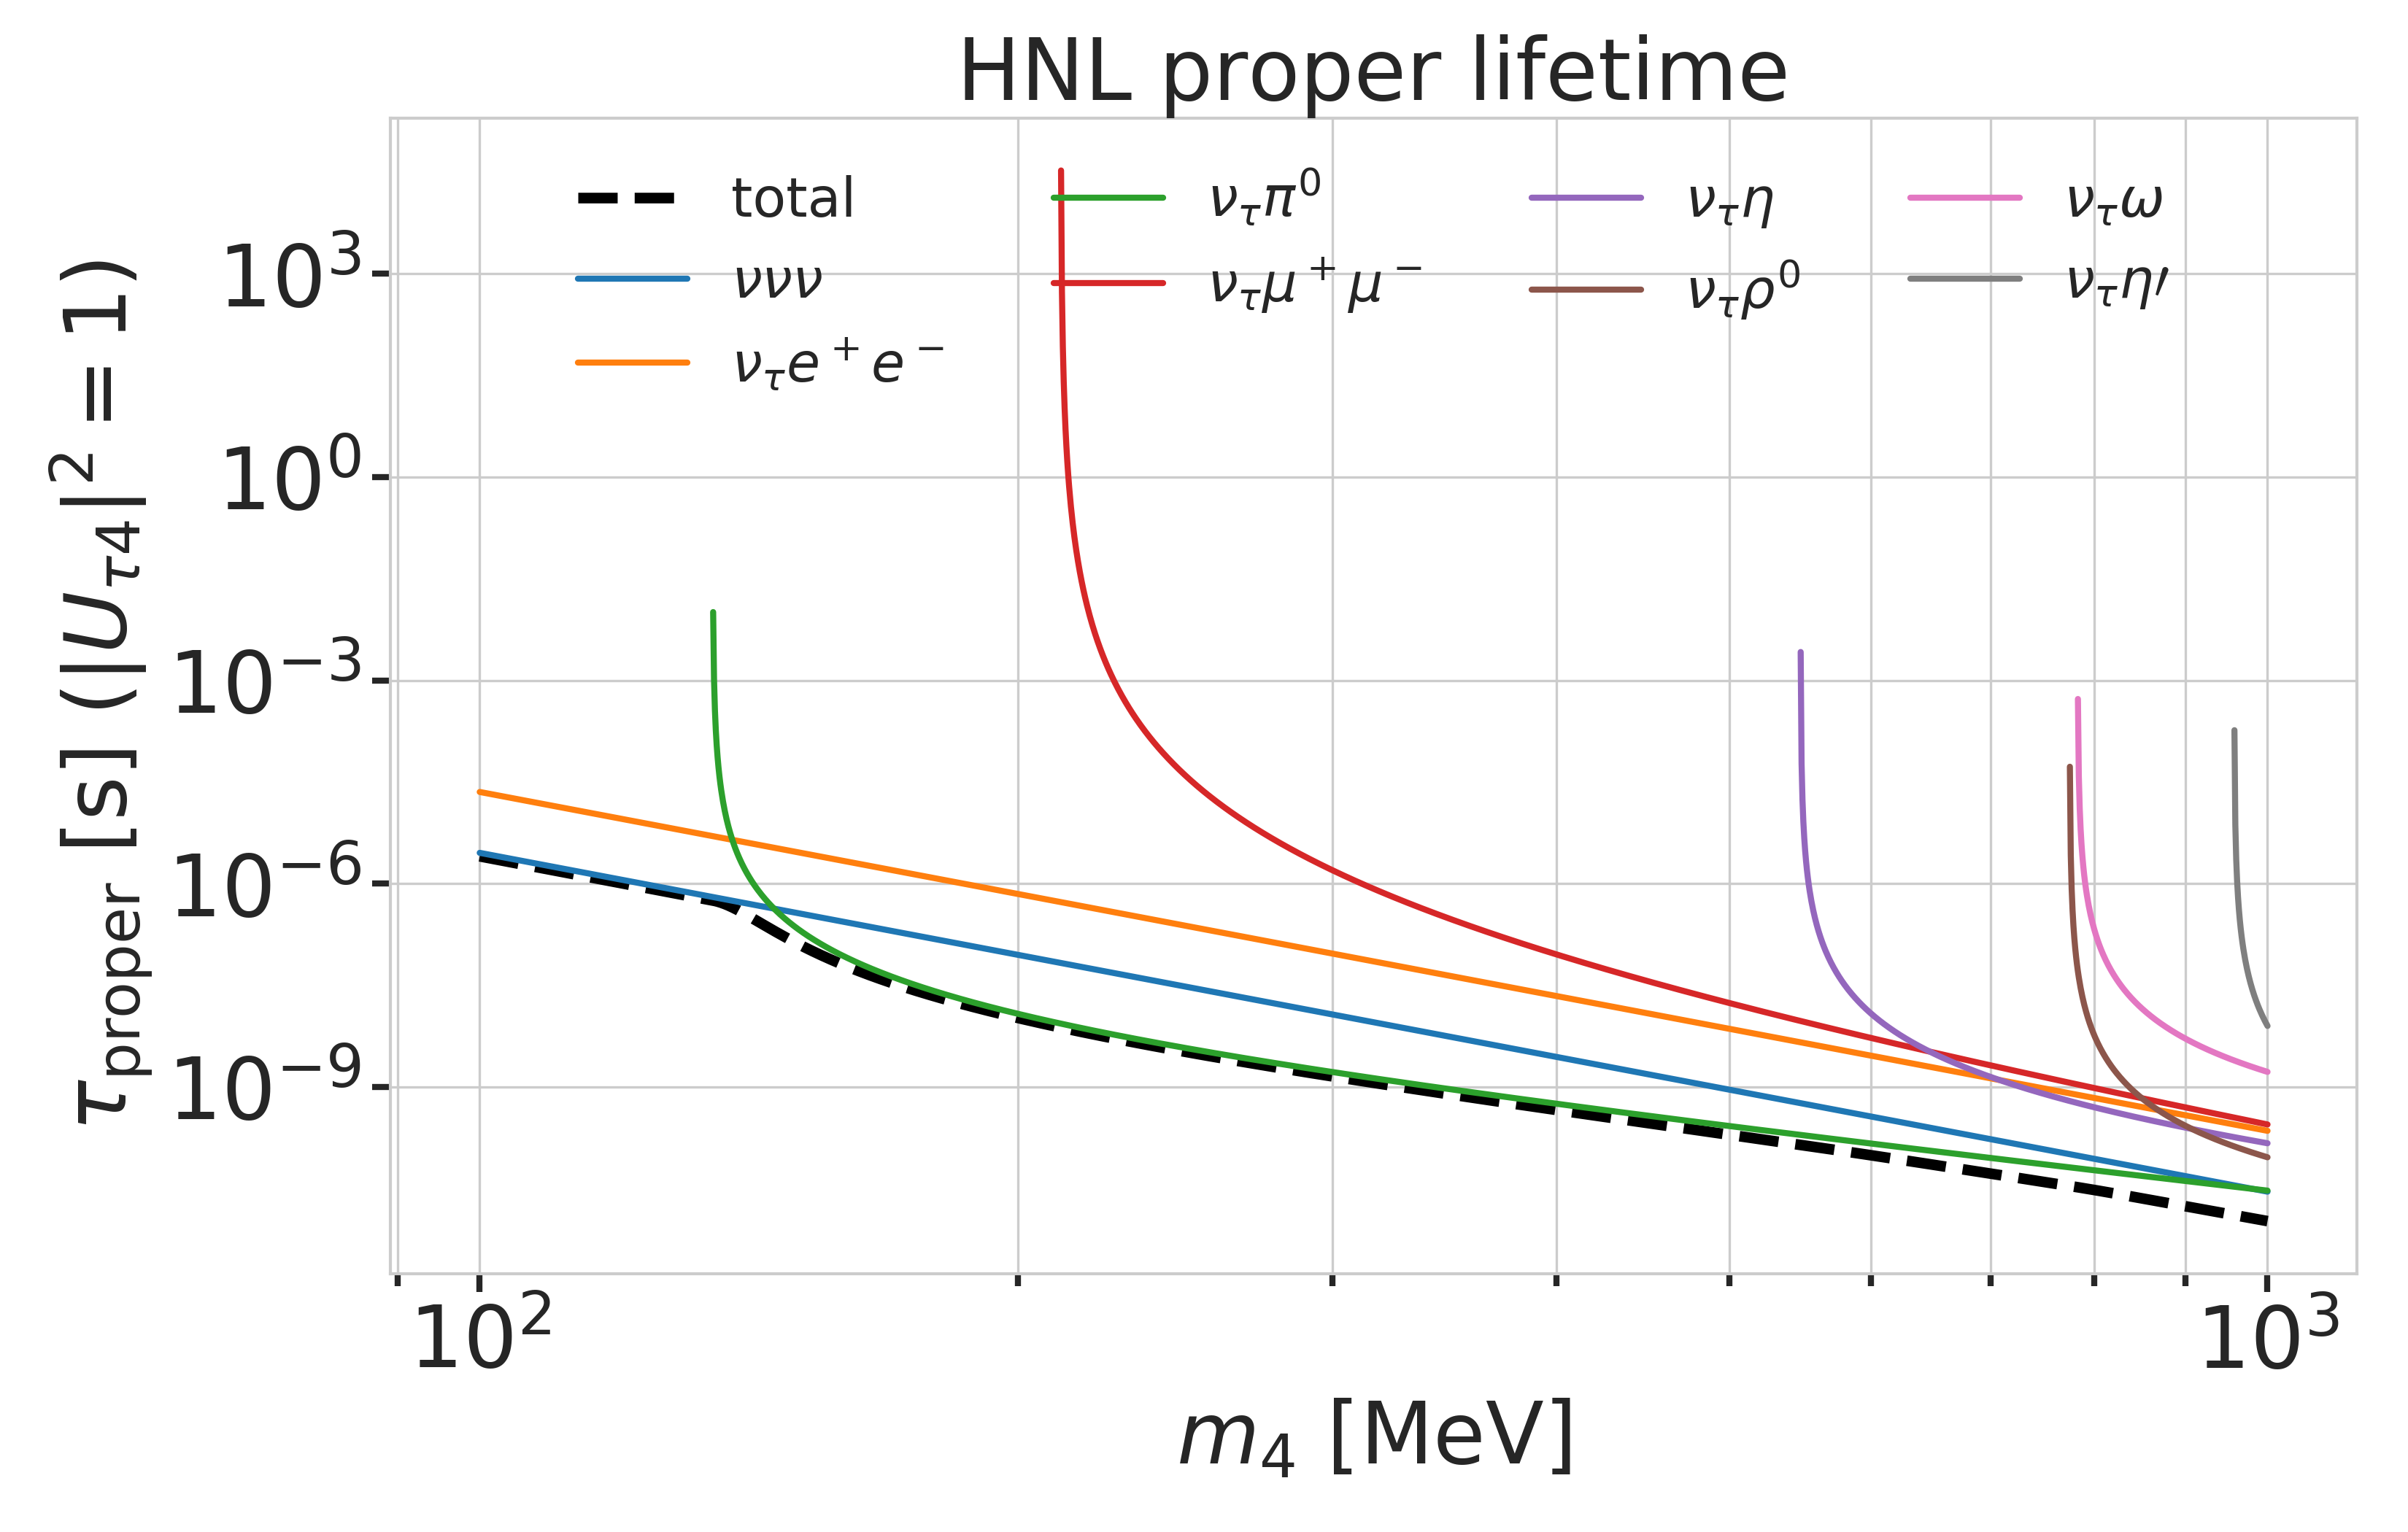
\includegraphics[width=.45\linewidth]{hnl_simulation/decay_theory/proper_lifetimes_up_to_1.0_GeV_log.png}
%     }
%     \caption{Branching ratios, decay widths, and proper lifetime of the HNL within the mass range considered, calculated based on the results from \sidecite{Coloma:2020lgy}. Given the existing constraints on $|U_{e4}|^{2}$ and $|U_{\mu4}|^{2}$, we consider that the corresponding decay modes are negligible.}
%     \labfig{hnl_decay_modes_log}
% \end{figure}

\begin{figure}
    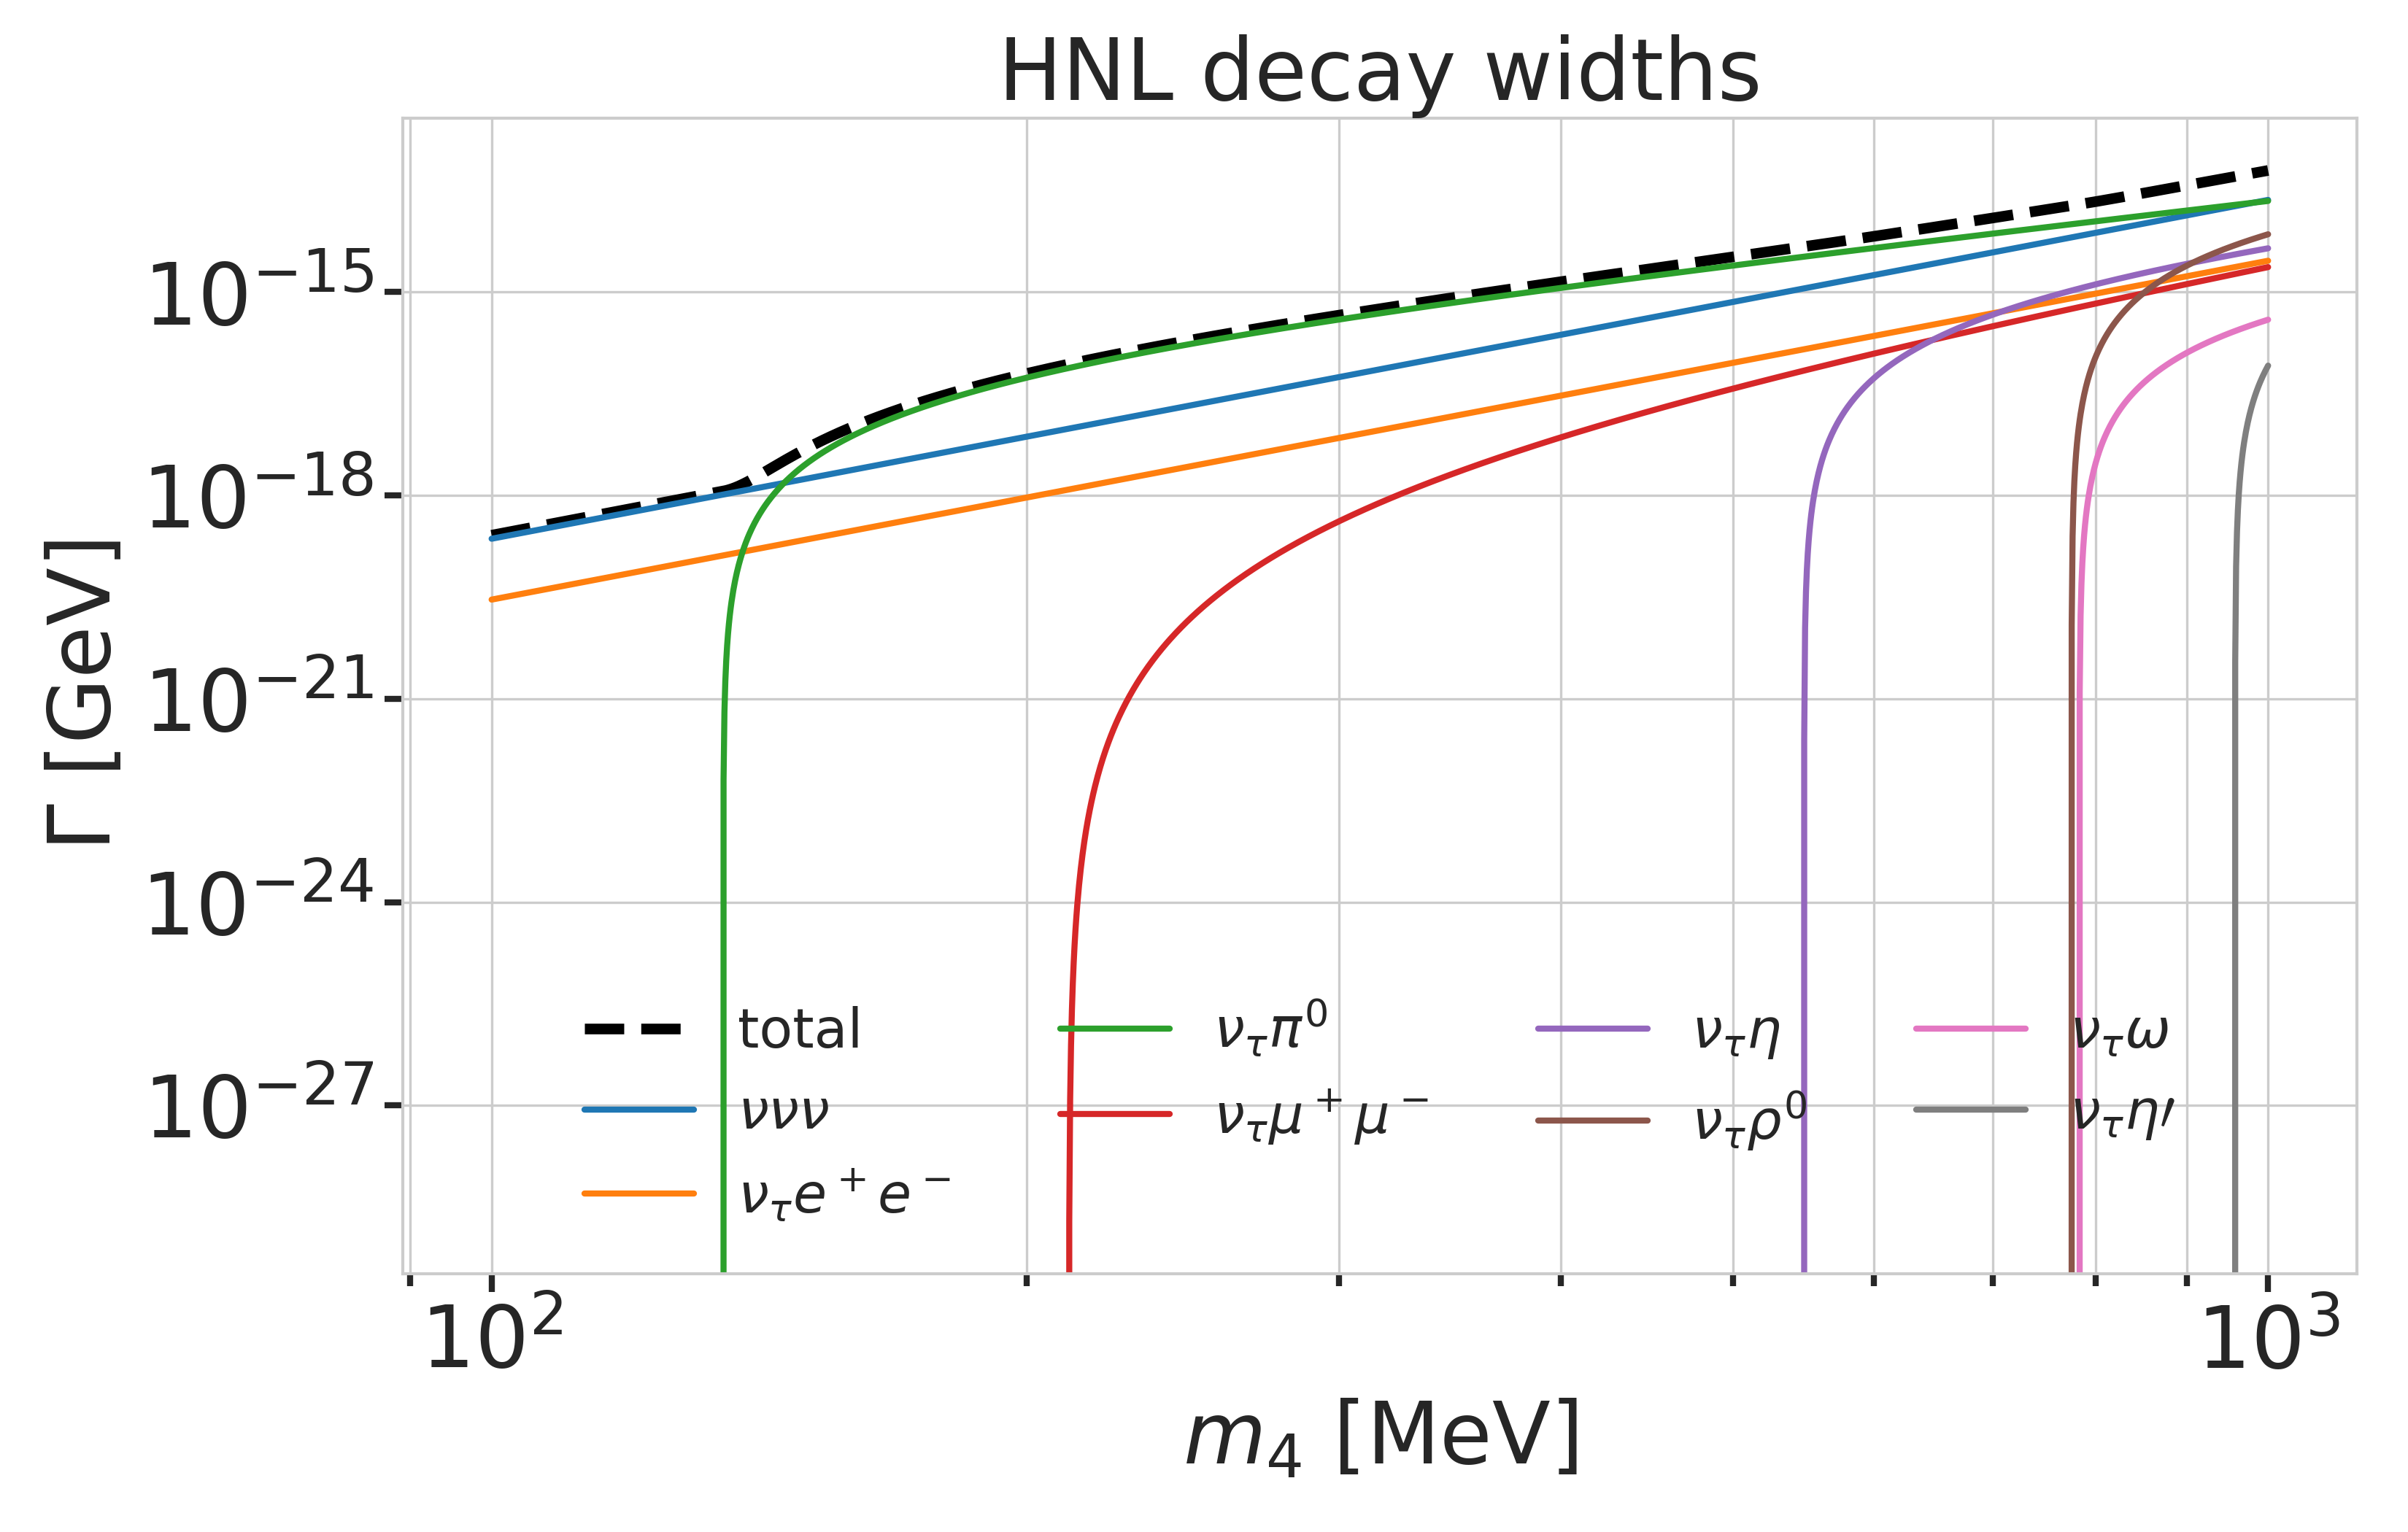
\includegraphics{hnl_simulation/decay_theory/hnl_decay_widths_up_to_1.0_GeV_log.png}
    \caption{Decay widths of the HNL within the mass range considered, calculated based on the results from \cite{Coloma:2020lgy}. Given the existing constraints on $|U_{e4}|^{2}$ and $|U_{\mu4}|^{2}$, we consider that the corresponding decay modes are negligible.}
    \labfig{hnl_decay_modes_log_decay_width}
\end{figure}


\subsection{Global Constraints on  mixing}


\section{Open Questions in Neutrino Particle Physics}
